% id: 41-h4
% book: 개념원리 중학 3-2 · 04 길이 구하기
% section: 핵심문제 익히기
% figure: crop:fig-41-h4.png
% answer: $4\sqrt{6}\mkern3mu \mathrm{cm}$
% answer_source: 본문 답
% variant_level: 0 (원본 전사)
% 이 파일은 build.mjs 가 items.json 에서 만든다. 고칠 때는 items.json 을 고친다.
\smash{\raisebox{1.5mm}{\dmkichul{개념원리 중학 3-2 41쪽 핵심문제 4}}}
\noindent\begin{minipage}[t]{0.58\linewidth}\vspace{0pt}\raggedright 오른쪽 그림과 같은 $\triangle\pt{ABC}$에서 $\seg{AB}=8\mkern3mu \mathrm{cm}$, $\angle\pt{B}=75^\circ$, $\angle\pt{C}=45^\circ$일 때, $\seg{BC}$의 길이를 구하시오.\end{minipage}\hfill\begin{minipage}[t]{0.4\linewidth}\vspace{0pt}\centering \setlength{\dmfigw}{80.1pt}\ifdim\dmfigw>\linewidth\setlength{\dmfigw}{\linewidth}\fi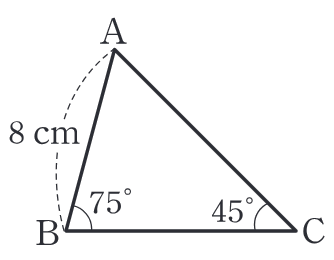
\includegraphics[width=\dmfigw]{figures/fig-41-h4.png}\end{minipage}\par
